\subsection{Overbelægning}
Definitionen af overbelægning er en overstigelse af indlagte patienter på en given afdeling ift. tilgængelige sengepladser. Overbelægning er estimeret til at være 85\% af det samlede antal sengepladser, herefter er det påvist at sandsynligheden for hospitalets mortalitet \fxnote{hyppigheden af dødsfald i en befolkning angives ved forholdet mellem antallet af døde inden for et givet tidsrum og størrelsen af befolkningen.} stiger 9\% sammenlignet med underbelægning. \citep{dodlighed2014} For at mindske konsekvenser af dette er det vigtigt at finde en ligevægt mellem over- og underbelægning.  

\noindent
Antallet af patienter, der indlægges varierer fra måned til måned, hvorfor tilgængeligheden af sengepladser varierere. Dette gør sig også gældende for flere forskellige afdelinger. 


\begin{figure}[H]
\centering
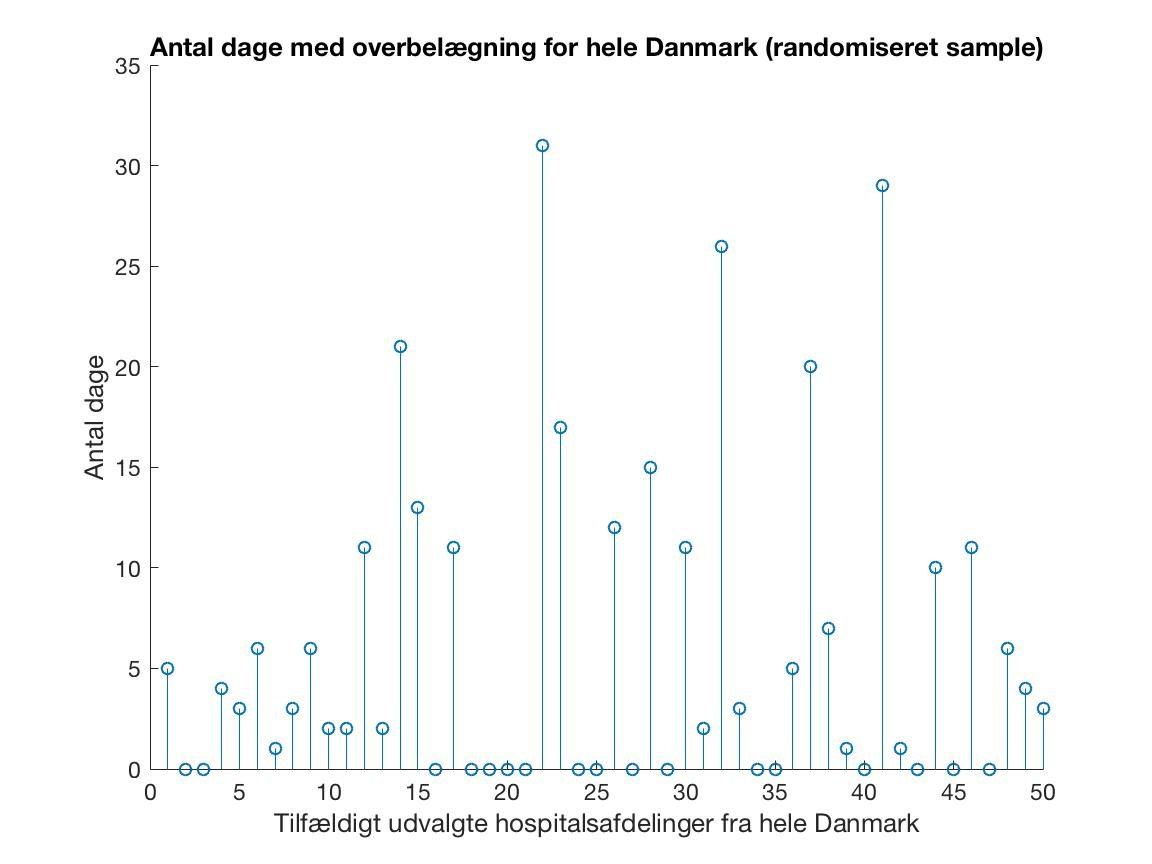
\includegraphics[width=0.5\textwidth]{overbelaegning_ran.fig}
\caption{ }
\label{Overbelaegning af patienter over hele Danmark}
\end{figure}
